\documentclass{article}
\usepackage{sbc-template}
\usepackage{graphicx,url}
\usepackage[utf8]{inputenc}
\usepackage[brazil]{babel}
\usepackage{subfigure}
\usepackage{amssymb}
     
\sloppy

\title{Análise de Centralidade em Redes Complexas}

\author{Rodrigo José Zonzin Esteves\inst{1}}


\address{Departamento de Computação -- Universidade Federal de São João del Rei\\}

\begin{document} 

\maketitle
     

\section{Dados}
A rede foi obtida através do portal “Stanford Network Analysis Project” e apresenta uma rede social virtual obtida por meio do Facebook. Os dados foram anonimizados, retirando-se o ID identificador do perfil real, e apresentam atributos como afinidade partidária - com uma máscara numérica para democratas e republicanos. \cite{McAuley2012}.  

\section{Análise}
\subsection{Centralidade por grau - Clustering}

Também conhecido como “Coeficiente de Clustering”. 
\begin{figure}[h!]
	\centering
	\caption{Vértices por Clustering}
	
	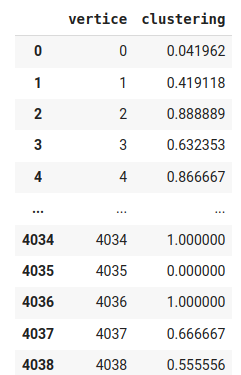
\includegraphics[height=5cm]{img/clustering}
	
	\label{fig:clustering}
\end{figure}


Observou-se $\hat{C} =   0.605547$ , $ \sigma = 0.214462$, $Q_{0.25}= 0.466667$ , $M_{c_v} = 0.600000$, $Q_{0.75}= 0.752381$. 
Os 10 vértices com maior centralidade estão apresentados na imagem a seguir. 

\subsection{Closeness}
Os vértices com maiores valores de Closeness são apresentados na tabela a seguir. 
\begin{figure}[h!]
	\centering
	\caption{10 vértices com maior Closeness}
	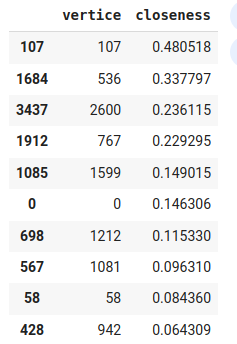
\includegraphics[height=5cm]{img/maioresCloseness}
	\label{fig:closeness}
\end{figure}


$Closeness_{avg} =   6.669574e-04$ , $\sigma = 1.164634e-02$, $ Q_{0.25} =  3.997507e-07$, $M =  2.918300e-06$ e $Q_{0.75} = 1.515292e-05$. 

\newpage 
\subsection{Betweenness}

\begin{figure}[h!]
	\centering
	\caption{10 vértices com maior Betweenness}
	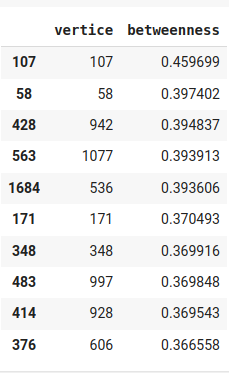
\includegraphics[height=5cm]{img/betweenness}
	\label{fig:betweenness}
\end{figure}
$Betweenness_{avg} = 0.276168$,  $\sigma = 0.036124$, $Q_{0.25} = 0.260348$, $M = 0.282457$ e $Q_{0.75} = 0.315001$. 


\subsection{\textit{Eigenvector}}

\begin{figure}[h!]
	\centering
	\caption{10 vértices com maior eigencentrality}
	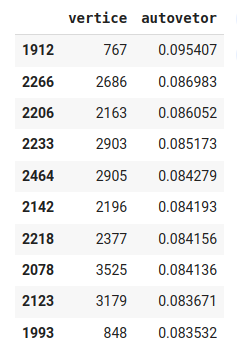
\includegraphics[height=5cm]{img/autovetor.png}
	\label{fig:autovetor}
\end{figure}

\section{Discussão}
O clustering se dá em função do grau de cada vértice, como na equação a seguir. 
Da análise realizada, observa-se que os 10 vértices com maior clustering têm coeficiente igual a 1. 
Matematicamente, 
$$C^{i}_{grau} = \frac{k_i}{n-1} = 1 \Longleftrightarrow k_i = n-1$$
Desse resultado, segue-se que a rede em análise apresenta vértices cuja conectividade é máxima (estão ligados a todos os demais vértices). 
Topologicamente, essa propriedade é interessante uma vez que esses vértices são capazes de atingir qualquer outro vértice de interesse. 

Ademais, no quartil superior, os vértices estão ligados a pelo menos 75\% da rede. 
De forma similar, esse é um valor expressivo e pode ser utilizado, por exemplo, caso não se soubesse a priori da existência de conectividade maximal em alguns vértices da rede -- escolhas ótimas, com custo unitário, para se atingir qualquer outro vértice da rede. 

A medida de Closeness apresenta a distância média entre um vértice $v$ e todos os demais $u \in V - \{v\}$ através do caminho mais curto. 
Essa medida é capaz de mensurar o quão rápido uma propriedade pode trafegar na rede. 

De acordo com a figura \ref{ref2}, os nós com maior closeness pertecem a clusters diferentes. 
Desse modo, tais vértices podem ser bastante influentes na velocidade de trafego de propriedades na rede, mas com maior influência ao seu cluster.  

A centralidade Betweenness quantifica como um nó age como ponte entre o caminho minimo de dois outros vértices. 
Essa métrica é capaz de aferir a influência que cada vértice sobre o fluxo de propriedade de uma rede. 

Diferentemente do closeness, a topologia da rede sugere que os vértices têm uma influência similar na propagação de propriedades sobre a rede. 
De fato, tomando o coeficiente de variação das duas centralidades, observamos $CV_{clos} = 17.4597$ e $CV_{bet} = 0.1307$, indicando que não há valores de betweenness que se destacam. 

A centralidade por autovetor (\textit{eigenvector centrality}) considera a conexão de um vértice a "vértices importantes" na rede. 
Isto é, quanto mais próximo de vértices importantes ele está, mais importante ele se torna -- e maior será sua centralidade por \textit{eigenvector}.

A figura \ref{fig:autovetor} apresenta os 10 vértices com maior centralidade por autovetor. 
Pode-se observar que os vértices estão dispostos um ao outro (entre 1912 e 2464). 
De maneira similar, a figura \ref{ref4} apresenta que o "vértice mais importante" é cercado por outros vértices importantes (sobrepostos em cor laranja) e seguidos por vértices de cor azul. 

As demais regiões da rede apresentam vértices pequenos, dos quais muitos se quer foram representados. 




\newpage
\section{Visualização da Rede}
As figuras a seguir apresentam atributos de centralidade da rede discricionados por tamanho e cor do vértice. 
Para cada figura, quanto maior o nó, maior é o respectivo atributo. 

\begin{figure}[htbp]
	\centering
    \caption{Centralidade por Autovetor}

	\subfigure[ref1][Grau]{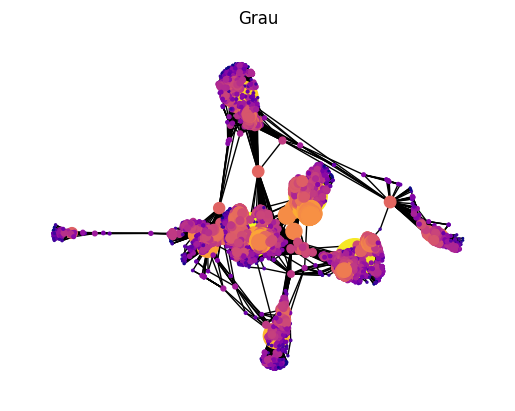
\includegraphics[height=8cm]{../plotGrau} \label{ref2}}
	\qquad

	\subfigure[ref2][Closeness]{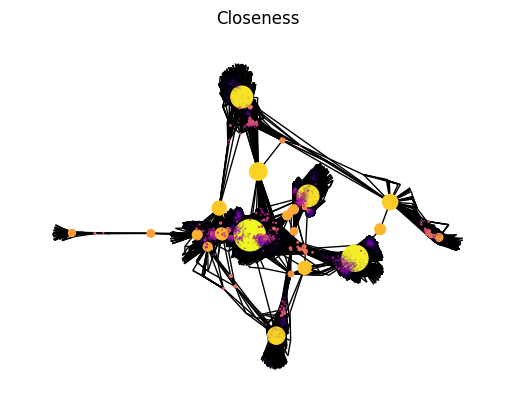
\includegraphics[height=8cm]{../plotCloseness}}
	\qquad 
\end{figure}

\begin{figure}
    \centering
	\subfigure[ref3][Betweenness]{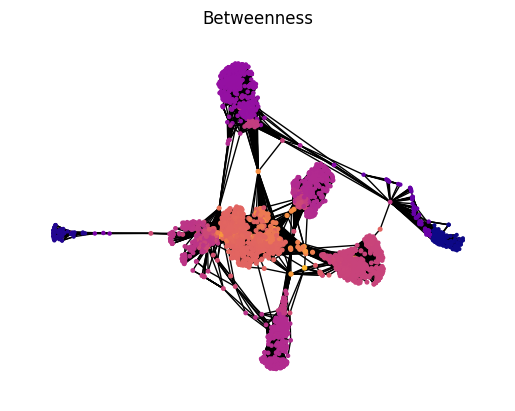
\includegraphics[height=8cm]{../plotBetweenness}}
 	\qquad

 	\subfigure[ref4][Autovetor]{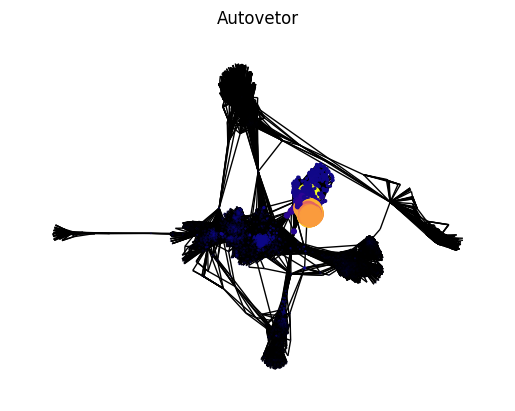
\includegraphics[height=8cm]{../plotAutovetor} \label{ref4}}
 	\qquad 

\label{fig:Centralidade}
\end{figure}

\newpage

\bibliographystyle{sbc}
\bibliography{sbc-template}

\end{document}
